\section{Finite Element Formulation}
\label{sct-FEF}
\LV is a finite element library. We need to formulate the mathematical problem related to Eq. \eqref{eq::ConLinMom-Diff} in the framework of the finite element method. In this section we introduce the continuous weak formulation and its approximation by the Galerkin method. After this, we will describe the nonlinear problem that has to be solved (using a Newton method) at each time step of the simulation. Its linearization is presented, and the Jacobian of the nonlinear operator is shown for each of the four constitutive laws.

\subsection{Weak formulation of the structural mechanic problem}
\label{sct-ContinuousWF}
In order to derive the weak formulation of the problem related to Eq. \eqref{eq::ConLinMom-Diff} we need first to define it. Fig. \ref{fig::Domain} represents the domain of the problem. The domain defined by the dashed line is the reference configuration \RefCon and the one delimited by the solid line is the current configuration \CurCon. The portion of the boundary $\Gamma _D$ is where Dirichlet boundary conditions are applied and $\Gamma_{N_i}$ ($i=1,2$) are the portions of $\partial \RefConE$ where Neumann boundary conditions are applied. It is worth to note that the mathematical structural dynamic problem is defined on \RefCon since \eqref{eq::ConLinMom-Diff} has been written in the Lagrangian framework.

\begin{figure}[h!]
  \centering
  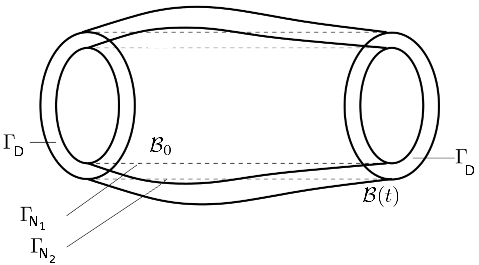
\includegraphics{images/Structure.pdf}
  \caption{Domain of the structural problem \eqref{eq::MathProb}}
  \label{fig::Domain}
\end{figure}

The differential problem is:
\begin{equation}
\left\{
\begin{array}{lllllll}
  \displaystyle \rho_0\frac{\partial^2\displL}{\partial t^2}=\rho_0\underline{b}+\text{Div}(\Piola) & \text{on} \quad \RefConE \vee t>0,\\
  \\
  \displL(0)=\displL_0 & \text{on} \quad \RefConE \vee t=0,\\
  \velL(0)=\velL_0 & \text{on} \quad \RefConE \vee t=0,\\
  \displL(t)=\underline{0} & \text{on} \quad \Gamma_D, \quad t>0,\\
  \Piola\underline{n}_1=\underline{0} & \text{on} \quad \Gamma_{N_1}, \quad t>0,\\
  \Piola\underline{n}_2=\underline{t}_0 & \text{on} \quad \Gamma_{N_2}, \quad t>0.\\
\end{array}\right.
\label{eq::MathProb}
\end{equation}
If we consider the equation of motion in \eqref{eq::MathProb}, multiply it by an arbitrary velocity field $\velwE$ and integrate the equation on \RefCon, we get:
\begin{equation}
  \displaystyle \int_{\RefConE}\rho_0\frac{\partial^2 \displL}{\partial t^2}\cdot\velwE\quad d\RefConE = \int_{\RefConE}\diver{(\Piola(\displL)}\cdot\velwE\quad d\RefConE + \int_{\RefConE}\rho_0\underline{b}\cdot\velwE\quad d\RefConE
  \label{eq::firstIntegral}
\end{equation}
Applying the divergence theorem to the first integral at the right hand side and taking into account the boundary conditions in \eqref{eq::MathProb} the integral relation \eqref{eq::firstIntegral} becomes:
\begin{equation}
  \begin{array}{lll}
    \displaystyle \int_{\RefConE}\rho_0\frac{\partial^2 \displL}{\partial t^2}\cdot\velwE\quad d\RefConE  & = \displaystyle - \int_{\RefConE}\Piola(\displL):\delOp\velwE\quad d\RefConE + \\
    \\
    & \displaystyle + \int_{\partial \RefConE}\underline{t}_0\cdot\velwE\quad d\partial\RefConE + \int_{\RefConE}\rho_0 \underline{b}\cdot\velwE\quad d\RefConE
    \end{array}
  \label{eq::secondIntegral}
\end{equation}
which can be written in this form,
\begin{equation}
  \begin{array}{lll}
    & \displaystyle \int_{\RefConE}\rho_0\frac{\partial^2 \displL}{\partial t^2}\cdot\velwE\quad d\RefConE  + \int_{\RefConE}\Piola(\displL):\dot{\F}\quad d\RefConE = \\
    \\
    & \displaystyle = \int_{\partial \RefConE}\underline{t}_0\cdot\velwE\quad d\partial\RefConE + \int_{\RefConE}\rho_0 \underline{b}\cdot\velwE\quad d\RefConE,
    \end{array}
  \label{eq::secondIntegral}
\end{equation}
having used the identity $\delOp\velwE = \dot{\F}$. The second term at the left hand side strictly depends on the adopted constitutive law. The reinterpretation of the arbitrary velocity $\velwE$ as a test function provides the weak formulation of the problem \eqref{eq::MathProb}.\\
Let $V$ be the following space of the vector fields,
\begin{equation}
  V(\RefConE)=\left\{\phi\in\left[H_{\Gamma_D}^1(\RefConE)\right]^3\right\}=\left\{\phi\in\left[H_{0}^1(\RefConE)\right]^3 s.t. \quad \phi=0 \quad\text{on}\quad\Gamma_D\right\}
  \label{eq::TestSpace}
\end{equation}
the weak formulation is:\\
 \\
\textit{Find $\displL=\displL(\posE,t)\in V$ such that $\displL(0)=\displL_0$, $\velL(0)=\velL_0$ and} :
\begin{equation}
  \begin{array}{lll}
    & \displaystyle \int_{\RefConE}\rho_0\frac{\partial^2 \displL}{\partial t^2}\cdot\phi\quad d\RefConE  + \int_{\RefConE}\Piola(\displL):\delOp\phi\quad d\RefConE = \\
    \\
    & \displaystyle = \int_{\partial \RefConE}\underline{t}_0\cdot\phi\quad d\partial\RefConE + \int_{\RefConE}\rho_0 \underline{b}\cdot\phi\quad d\RefConE \qquad \forall \phi\in V, \quad \forall t>0.
    \end{array}
  \label{eq::WF}
\end{equation}
For the case with non-homogeneous Dirichlet boundary conditions, the interested reader may refer to \cite{Hughes}.

\subsection{Discrete weak formulation}
\label{sct-DiscreteWF}
The discrete weak formulation is obtained by considering a conforming triangulation ($T_h$) of the domain \RefCon, which leads to an approximation of it $\RefConE^h$, and by considering a subspace $V_h\subseteq V$ of finite dimension. This subspace is composed by the piecewise continuous polynomial functions over $\RefConE^h$, in formulae:
\begin{equation}
  Q_h(T_h)=\left\{\phi_h \in C^0(\RefConE^h), \phi_{h|K} \in \mathbb{P}^N\big(K\big), \forall K \in T_h\right\},
  \label{eq::SpaceDiscrete}
\end{equation} 
where $K$ is an element of the triangulation $T_h$. The discrete functional space to approximate the solution of the structural mechanic problem is $V_h=\left[Q_h(T_h)\right]^3$. Moreover, any function $\phi_h\in V_h$ has to satisfy:
\begin{displaymath}
  \phi_h=0 \qquad \text{on}\quad\Gamma_D.
\end{displaymath}
The discrete formulation follows directly from the continuous one (Eq. \eqref{eq::WF}),\\
\textit{Find $\displL_h=\displL_h(\posE,t)\in V_h(\RefConE^h)$ such that $\displL(0)=\displL_{0h}$, $\velL(0)=\velL_{0h}$ and} :
\begin{equation}
  \begin{array}{lll}
    & \displaystyle \int_{\RefConE^h}\rho_0\frac{\partial^2 \displL_h}{\partial t^2}\cdot\phi_h\quad d\RefConE^h  + \int_{\RefConE^h}\Piola(\displL_h):\delOp\phi_h\quad d\RefConE^h = \\
    \\
    & \displaystyle = \int_{\partial \RefConE^h}\underline{t}_{0h}\cdot\phi_h\quad d\partial\RefConE^h + \int_{\RefConE^h}\rho_0 \underline{b}_h\cdot\phi_h\quad d\RefConE^h \qquad \forall \phi_h\in V_h, \quad \forall t>0.
    \end{array}
  \label{eq::DWF}
\end{equation}
The functions $\displL_{0h}$,$\velL_{0h}$,$\underline{t}_{0h}$,$\underline{b}_h$ are suitable approximations of the initial and boundary data in $V_h$.\\
As it is usually done in the finite element method, we consider a basis $\left\{\Phi_h\right\}_{i=1}^{N_h}$ where $N_h=\text{dim}V_h$  and the solution $\displL_h$ will be given by:
\begin{equation}
  \displaystyle \displL_h(\posE,t)= \sum_{i=1}^{N_h}\displL_h^i(t)\Phi_i(\posE).
  \label{eq::DiscreteSolution}
\end{equation}
Introducing \eqref{eq::DiscreteSolution} in \eqref{eq::DWF} we get the algebraic system:
\begin{equation}
  \mass\frac{\partial^2\vectL}{\partial t^2}+\StiffVect = \underline{f},
  \label{eq::GeneralSystem}
\end{equation}
where $\vectL \in \RN$ is the vector of the nodal displacement $\left\{\displL_h^i(t)\right\}_{i=1}^{N_h}$. It is worth to note that equation \eqref{eq::GeneralSystem} is still continuous in time and it must be discretized properly. The different terms in \eqref{eq::GeneralSystem} are:
\begin{itemize}
  \item \mass: the mass matrix defined as: $\displaystyle M_{ij}=\int_{\RefConE}\rho_0\phi_i\phi_j\quad d\RefConE^h$;
  \item[]
  \item $\StiffVect$: the stiffness vector defined as: $\displaystyle \left(\StiffVect\right)_{j=1\ldots N_h}=\int_{\RefConE^h}\Piola\left(\sum_{i=1}^{N_h}\displL_h^i(t)\Phi_i(\posE)\right):\delOp\Phi_j\quad d \RefConE^h$;
  \item[]
  \item $\underline{f}$ is the forcing term defined as: $\displaystyle (\underline{f})_{j=1\ldots N_h}=\int_{\RefConE^h}\sum_{i=1}^{N_h}t_{0i}\Phi_i\Phi_j+b_i\Phi_i\Phi_j\quad d\RefConE^h$.
\end{itemize}
The algebraic system \eqref{eq::GeneralSystem} is nonlinear in the variable $\vectL$ and the Newton method is used to solve it at each time step.

\subsection{Linearization}
\label{sct-Linear}
In this report we will not address the discretization in time of equation \eqref{eq::GeneralSystem}. It is carried out by another class implemented in \LV, called \textit{TimeAdvance}. For this reason, the interested reader may refer to the documentation of that class. In the following we will describe the linearization of the nonlinear problem \eqref{eq::GeneralSystem} at each time step. We suppose that the displacement field is known at a certain time $t=n$ is called it $\vectL^n$. Moreover, let us suppose that the corresponding velocity and acceleration fields ($\velVect^n$ and $\acc^n$ respectively) have been computed according to the time marching procedure used. We want to compute the displacement vector at time $t=n+1$. The general form of the nonlinear algebraic problem is
\begin{equation}
\xi\mass\vectL^{n+1}+\StiffDiscr{n+1}=\underline{G}\left(\underline{f}^{n+1},\vectL^n,\velVect^n,\acc^n\right),
\label{eq::SystemN}
\end{equation}
where $\xi$ is related with the time marching procedure and $\underline{G}$ is the right hand side of \eqref{eq::SystemN}. Let us define and operator $\LE:\RN\to\RN$ as:
\begin{equation}
  \LE:\quad\xi\mass\vectL^{n+1}+\StiffDiscr{n+1}-\underline{G}.
\label{eq::NonLinearOperator}
\end{equation}
According to \eqref{eq::NonLinearOperator}, finding $\vectL^{n+1}:\LE\left(\vectL^{n+1}\right)=0$ is equivalent to solve \eqref{eq::SystemN}. We apply the Newton method to find the roots of \Lne. Doing this, the unknown of the problem at each Newton iteration $k$ is the displacement $\vectL^{k}$ which is set initially to $\vectL^{n}$. It is necessary to introduce the Jacobian of \Lne, $J_{\text{\Lne}}(\vectL^{k}) = \text{D}\LE(\vectL^{k})$ and the increment of solution $\delta\vectL^{k} = \vectL^{k+1} - \vectL^{k}$.\\
Hence the problem becomes:\\

Let $\vectL^{0} \in$ $\RN$ be given (for instance from the previous time-step), 
iterate for $k$ = 1, 2, ...  until convergence:

\begin{equation}
 \boxed{
 \begin{array}{lc}
  \mbox{solve} & \hspace{2cm} \text{J}_{\LE}(\vectL^{k})\delta\vectL^{k} = -\LE(\vectL^{k})\,,\\
  \mbox{define} & \hspace{2cm} \vectL^{k + 1} = \vectL^{k} + \delta\vectL^{k}\,,
 \end{array}
 }
 \label{RichardsonI}
\end{equation}

and set $\vectL^{n+1} = \vectL^{k+1}$.
The test for convergence is the infinity norm of the residual. In particular, defining a tolerance 
$\varepsilon_{R}$ = $\overline{\varepsilon_{R_{abs}}}$ + $\mid{\LE(\vectL^{0})}\mid\overline{\varepsilon_{R_{rel}}}$
the stopping criterion for the Newton method is the following:

\begin{equation}
 \parallel{\LE(\vectL^{k})}\parallel_{\text{L}^{\infty}(\widehat{\Omega})}\,\,<\,\,\varepsilon_{R}\,.
\end{equation}
From the mathematical point of view, the Jacobian of \Lne is computed using the Gateaux derivatives. It can be shown (see \cite{Deluca} for details) that:
\begin{equation}
  \text{D}\LE(\vectL^{k})\delta\vectL^{k}=\left[\xi\mass+\text{D}\StiffDiscr{k}\right]\delta\vectL^{k}.
\label{eq::GeneralJacobian}
\end{equation}
From the equation above, it is clear that the main issue related to the computation of the Jacobian of the operator \Lne is the computation of the second term in parentesis. In particular, in \cite{Deluca} it is shown that
\begin{equation}
  \text{D}\StiffDiscr{k}\delta\vectL^{k} = \int_{\RefConE^h}D\Piola\left(\vectL^{k}\right)\delta\vectL^{k}:\delOp\Phi d\RefConE^h,
\label{eq::LinearizationK}
\end{equation}
where $\Phi$ is a generic function in $V_h$.\\
In the following subsections, the exact expression of the terms $D\Piola\left(\vectL^{k}\right)\delta\vectL^{k}$ for all the four structural models described in Section \ref{sct-Constitutive} is reported. For detailed comparisons, the reader may refer to \cite{Deluca}.

\subsubsection{St. Venant-Kirchhoff and Linear Elastic models}
Recalling the definition \eqref{eq::SVK-P-displ} of \Piola in the case of the St. Venant-Kirchhoff model, its Jacobian is
\begin{equation}
 \begin{array}{lllllllllll}
  \displaystyle \text{D}\Piola(\Spost)[\delta\Spost] & = \displaystyle \lambda(\delOp\cdot\delta\Spost) + \mu(\delOp\delta\Spost + (\delOp\delta\Spost)^T) + \lambda\delOp\Spost:\delOp\delta\Spost +\\
\\
                                           & \displaystyle + \lambda(\delOp\cdot\Spost)\delOp\delta\Spost + \lambda(\delOp\cdot\delta\Spost)\delOp\Spost + \frac{\lambda}{2}(\delOp\delta\Spost:\delOp\Spost)\delOp\Spost +\\
\\
                                           & \displaystyle + \frac{\lambda}{2}(\delOp\Spost:\delOp\delta\Spost)\delOp\Spost + \frac{\lambda}{2}(\delOp\Spost:\delOp\Spost)\delOp\delta\Spost +\\
\\
                                           & \displaystyle + \mu(\delOp\Spost)^{\text{T}}\delOp\delta\Spost + \mu(\delOp\delta\Spost)^{\text{T}}\delOp\Spost + \mu\delOp\Spost\delOp\delta\Spost + \mu\delOp\delta\Spost\delOp\Spost +\\
\\
                                           & \displaystyle + \mu\delOp\Spost(\delOp\delta\Spost)^{\text{T}} + \mu\delOp\delta\Spost(\delOp\Spost)^{\text{T}} + \mu\delOp\delta\Spost(\delOp\Spost)^{\text{T}}\delOp\Spost +\\
\\
                                           & \displaystyle + \mu\delOp\Spost(\delOp\delta\Spost)^{\text{T}}\delOp\Spost + \mu\delOp\Spost(\delOp\Spost)^{\text{T}}\delOp\delta\Spost.
 \end{array}
\label{eq::SVK-Jacobian}
\end{equation}
The replacement of \eqref{eq::SVK-Jacobian} in \eqref{eq::LinearizationK} provides the linearization of the stress tensor needed in \eqref{eq::GeneralJacobian}. For the linear elastic model, the first Piola-Kirchhoff tensor is a linear tensorial function of the displacement field and, for this reason, its Jacobian is equal to the tensor itself (Eq. \eqref{eq::LE-P}). 

\subsubsection{Neohookean model}
In the case of Neohookean materials, the tensor \Piola is the sum of the isochoric and volumetric part. Because of the presence of $\F^{-T}$ in the expression of \Piola (Eq. \eqref{eq::NH-P}), its Jacobian will be computed in terms of $\F,\cofF$, where \cofF is the cofactor matrix of \F (defined as $\cofF=J\F^{-T}$, where $J=\text{det}\F$). Because of the linearity of the Gateaux derivative operator,
\begin{equation}
\text{D}\Piola(\F)[\GradSpost]=\Piola_{isochoric}(\F)[\GradSpost]+\Piola_{volumetric}(\F)[\GradSpost].
\end{equation}
The firs term is:
\begin{equation}
  \begin{array}{llllllllllll}
    \text{D}\Piola_{isochoric}(\F)[\GradSpost] = & \displaystyle -\frac{2}{3}J^{-\frac{5}{3}}\left(\cofF:\GradSpost\right)\F +\\
    \\
    & \displaystyle + \frac{2}{9}\mu J^{-2}I_{\C}\left(\cofF:\GradSpost\right)\cofF + \\
    \\
    & \displaystyle - \frac{2}{3}\mu J^{-\frac{5}{3}}\left(\F:\GradSpost\right)\cofF + \\
    \\
    & \displaystyle + \mu J^{-\frac{2}{3}}\GradSpost + \\
    \\
    & \displaystyle + \frac{\mu}{3}J^{-2}I_{\C}\cofF\GradSpost^T\cofF.
\end{array}
\label{eq::IsoPartDP-neo}
\end{equation}
The volumetric term is:
\begin{equation}
  \begin{array}{lll}
    \text{D}\Piola_{volumetric}(\F)[\delta\Spost] = & \displaystyle + \frac{\kappa}{2}\left(2J^2-J+1\right)\left[\F^{-T}:\GradSpost\right]\F^{-T}\\
    \\
    & \displaystyle + \frac{\kappa}{2}\left(J-J^2-\text{ln}(J)\right)\F^{-T}\GradSpost^T\F^{-T}. \\
\end{array}
\label{eq::VolPartDP-neo}
\end{equation}
In the previous formulae $\mu$ and $\kappa$ are the shear and bulk modulus respectively.

\subsubsection{Exponential model}
In this case, the same approach followed for the Neohookean material is used. In particular, the isochoric part becomes:
\begin{equation}
  \begin{array}{llllllllllllll}
    \text{D}\Piola_{isochoric}(\F)[\GradSpost] = & \displaystyle -\frac{2}{3}\alpha\term J^{-\frac{5}{3}}\left(1+\gamma I_{\C}\right)\left[\cofF:\GradSpost\right]\F +\\
    \\
    & \displaystyle + 2\alpha\gamma \term J ^{-\frac{4}{3}}\left(\F:\GradSpost\right)\F + \\
    \\
    & \displaystyle + \frac{2}{9}\alpha\term J^{-2}I_{\C}\left(1+\gamma I_{\C}\right)\left(\cofF:\GradSpost\right)\cofF + \\
    \\
    & \displaystyle - \frac{2}{3}\alpha\term J^{-\frac{5}{3}}\left(1+\gamma I_{\C}\right)\left(\F:\GradSpost\right)\cofF \\
    \\
    & \displaystyle + \alpha\term J^{-\frac{2}{3}}\GradSpost + \\
    \\
    & \displaystyle + \frac{\alpha}{3}\term J^{-2}I_{\C}\cofF\GradSpost^T\cofF.
\end{array}
\label{eq::IsoPartDP-exp}
\end{equation}
The volumetric part is the same as \eqref{eq::VolPartDP-neo} since the Neohookean and Exponential models have the same volumteric term (Eq. \eqref{eq::NH-P}-\eqref{eq::EXP-P}).
